\documentclass[a4paper]{article}
%% Jose Javier Gonzalez Ortiz %%
%% Plantilla Latex generica   %%
%% 2014-11-08                 %%


% Generic Pakages
    \usepackage[utf8]{inputenc}                         % For Spanish characters
    \usepackage[english]{babel}               % Spanish hyphenation and document rules
    \usepackage{amsmath}                                % Standard math packages
    \usepackage{graphicx}                               % Image insertion.
    \usepackage{tikz}
    \usepackage{caption,subcaption}                     % For custom caption environments

    \usepackage{booktabs}                               % Beautiful Tables
    \usepackage{hyperref}                               % For linked references and URLinks
    \usepackage{fancyhdr}                               % Custom headers and footers
    \usepackage{appendix}                               % Enables appendices
    \usepackage{pdfpages}                               % Insert pdfs
    \usepackage{array}                                  % Enables array features
    \usepackage{algorithm}
    \usepackage[noend]{algpseudocode}
    \usepackage{eqparbox}
    \makeatletter
    \def\BState{\State\hskip-\ALG@thistlm}
    \makeatother
    %\usepackage[americanvoltages, europeancurrents, americanresistors, cuteinductors]{circuitikz}                          % Circuit Graphics
    \usepackage{mathtools}
    \usepackage{amsthm}
    
%Additional Features
    \usepackage{lipsum}                                 % Used for inserting dummy 'Lorem ipsum' text into the template
    \usepackage{enumerate}                              % Custom numerate, useful for i,ii,iii... I,II,III...
    \usepackage{sectsty}                                % Allows customizing section commands
    \usepackage{todonotes}                              % useful for leaving todonotes
    \usepackage[space]{grffile}                         % insert files with spaces
     %\usepackage{microtype}                             % Beatify engine
    %\usepackage[superscript]{cite}                     % CIting with superscript numerals
    %\usepackage{xcolor}                                    % Required for inserting color
    %\usepackage[usenames,dvipsnames]{color}                % Required for custom colors
    %\usepackage{xargs}                                 % Expanded arguments features
    %\usepackage{fix-cm}                                 % Computer-Modern at arbitrarysizes
    \usepackage{siunitx}                               % For SI Units
    %\usepackage{eurosym}                                % Eurosymbol
    %\usepackage{pdflscape}                              % enables landscape for pdfs
    %\usepackage{longtable}                              % Tables than span multipages

% Custom Settings
    % \decimalpoint                                       % American Decimal Point instead of Spanish comma

    % Margins
        \topmargin      = -0.45in
        \evensidemargin = 0in
        \oddsidemargin  = 0in
        \textwidth      = 6.5in
        \textheight     = 9.0in
        \headsep        = 0.25in

    \pagestyle{fancy}
    \lhead{\HWAuthorName}
    \chead{}
    \rhead{\HWClass : \HWTitle}
    \lfoot{}
    \cfoot{\thepage}
    \rfoot{}
    
    \renewcommand\headrulewidth{0.4pt} % Size of the header rule
    \renewcommand\footrulewidth{0.4pt} % Size of the footer rule

    \numberwithin{equation}{section} % Number equations within sections (i.e. 1.1, 1.2, 2.1, 2.2 instead of 1, 2, 3, 4)
    \numberwithin{figure}{section} % Number figures within sections (i.e. 1.1, 1.2, 2.1, 2.2 instead of 1, 2, 3, 4)
    \numberwithin{table}{section} % Number tables within sections (i.e. 1.1, 1.2, 2.1, 2.2 instead of 1, 2, 3, 4)

    \renewcommand{\labelitemi}{$\bullet$}                       %%bullet1 circle
    \renewcommand{\labelitemii}{\leavevmode \hbox to
    1.2ex {\hss \vrule height .9ex width .7ex depth -.2ex\hss }} %%bullet2 box

    \newcommand{\ul}[1]        {\underline{\smash{#1}}}         %%closer underline
    \newcommand{\gm}[1]         {\guillemotleft #1\guillemotright}  %$ pretty <<sth>>$

    \DeclarePairedDelimiter\floor{\lfloor}{\rfloor}
    \DeclarePairedDelimiter\ceil{\lceil}{\rceil}

%%%%%%%%%%%%%%%%%%%%%%%%%%%%%%%%%%%%%%%%%%%%%%%%%%%%%%%%%%%%%%%%%%%%%%%%%%%%%%%%%%
%%%                             CODIGO                                         %%%
%%%%%%%%%%%%%%%%%%%%%%%%%%%%%%%%%%%%%%%%%%%%%%%%%%%%%%%%%%%%%%%%%%%%%%%%%%%%%%%%%%

% Code insertion
    \usepackage{listings}                               % Main package for inserting code
    \usepackage{courier}                                % For using the courier font

    \AtBeginDocument{\numberwithin{lstlisting}{section}}  % Number listings within sections (i.e. 1.1, 1.2, 2.1, 2.2 instead of 1, 2, 3, 4)
    
    %%\captionsetup[lstlisting]{font={small,tt}}            %  Listings Font Size
    
    \renewcommand{\lstlistingname}{Código}              % For Codigo caption (requires caption package)

    \definecolor{background}{gray}{.98}                 % Background color definition
    \definecolor{comments}{RGB}{51,102,0}               % Comments   color definition
    \definecolor{keywords}{RGB}{0,0,120}                % Keywords   color definition
    \definecolor{keywords2}{RGB}{204,0,102}             % Keywords2  color definition
    \definecolor{numbers}{RGB}{127, 0, 127}             % Keywords2  color definition

    \definecolor{Maroon}{RGB}{128, 0, 0}

       % morekeywords={add,sub,mul,mulu,nand,sll,sra,srl,sltu,addi,sw,lw,beq,jarl,lui},
    \lstdefinelanguage{ICAI-RiSC-16}
   {morekeywords={add,sub,mul,mulu,nand,sll,sra,srl,sltu,addi,sw,lw,beq,jalr,lui,la,med},
        sensitive=false,
        morecomment=[l]{\#},
        morecomment=[l][\color{Maroon}]{.},
        morekeywords=[2]{r0, r1, r2, r3, r4, r5, r6, r7},
        keywordstyle=[2]{\color{violet}},
        % literate=%
        %    *{0}{{{\color{red!20!violet}0}}}1
        %     {1}{{{\color{red!20!violet}1}}}1
        %     {2}{{{\color{red!20!violet}2}}}1
        %     {3}{{{\color{red!20!violet}3}}}1
        %     {4}{{{\color{red!20!violet}4}}}1
        %     {5}{{{\color{red!20!violet}5}}}1
        %     {6}{{{\color{red!20!violet}6}}}1
        %     {7}{{{\color{red!20!violet}7}}}1
        %     {8}{{{\color{red!20!violet}8}}}1
        %     {9}{{{\color{red!20!violet}9}}}1
        %morecomment=[s]{/*}{*/},
        %morestring=[b]"
    }


    \lstset{
        frame=Ltb,
        framerule=0pt,
        aboveskip=0.5cm,
        framextopmargin=3pt,
        framexbottommargin=3pt,
        framexleftmargin=0.4cm,
        framesep=0pt,
        rulesep=.4pt,
        backgroundcolor=\color{background},
        rulesepcolor=\color{black},
        rulecolor=\color{black},
        %
        stringstyle=\ttfamily,
        basicstyle=\small\ttfamily,
        commentstyle=\itshape\color{comments},
        keywordstyle=\bfseries\color{keywords},
        %
        numberstyle=\tiny,
        numbers=left,
        numbersep=15pt,
        numberfirstline = false,
        %
        breakatwhitespace=false,         % sets if automatic breaks should only happenat whitespace
        breaklines=true,                 % sets automatic line breaking
        captionpos=b,                    % sets the caption-position to bottom
        escapeinside={<@}{@>},            % if you want to add LaTeX within your code
        keepspaces=true,                 % keeps spaces in text, useful for keepingindentation of code (possibly needs columns=flexible)
        showspaces=false,                % show spaces everywhere adding particularunderscores; it overrides 'showstringspaces'
        showstringspaces=false,          % underline spaces within strings only
        showtabs=false,                  % show tabs within strings adding particularunderscores
        stepnumber=1,                    % the step between two line-numbers. If it's1, each line will be numbered
        tabsize=2,                       % sets default tabsize to 2 spaces
    }
    

    \lstdefinestyle{customvhdl}{
        language=vhdl,                              % Language
        morekeywords = {},
        morestring=[b][\color{numbers}]',
        morestring=[b][\color{numbers}]",
        emph={std_logic,std_logic_vector,integer,unsigned,to_unsigned},
        emphstyle={\color{keywords2}\bfseries},%
        %deletekeywords={...},            % if you want to delete keywords from the given language
    }

    \lstdefinestyle{customc}{
        language = C
    }

    \lstset{language = ICAI-RiSC-16}



    % Grey scale definitions - Printing
    %\definecolor{background}{gray}{.98}
    %\definecolor{comments}{gray}{.45}
    %\definecolor{keywords}{gray}{.25}


%%%%%%%%%%%%%%%%%%%%%%%%%%%%%%%%%%%%%%%%%%%%%%%%%%%%%%%%%%%%%%%%%%%%%%%%
%%%%%%%%%%%%%%%%%%%%%%       HERE BE DRAGONS        %%%%%%%%%%%%%%%%%%%%
%%%%%%%%%%%%%%%%%%%%%%%%%%%%%%%%%%%%%%%%%%%%%%%%%%%%%%%%%%%%%%%%%%%%%%%%
%
%%%%%%%%%%%%%%%%%%%%%%%%%%%%%%%%%%%%%%%%%%%%%%%%%%%%%%%%%%%%%%%%%%%%%%%%
%%%% Paragraph separation
%\setlength{\parskip}{.5em}
%%%%%%%%%%%%%%%%%%%%%%%%%%%%%%%%%%%%%%%%%%%%%%%%%%%%%%%%%%%%%%%%%%%%%%%%
%%%% Table separation
%\renewcommand{\arraystretch}{1.3}
%%%%%%%%%%%%%%%%%%%%%%%%%%%%%%%%%%%%%%%%%%%%%%%%%%%%%%%%%%%%%%%%%%%%%%%%
%%%% 9+ Arguments functions
%\newcommand{\function}[9]{%
%        \def\tempa{#1}%
%        \def\tempb{#2}%
%        \def\tempc{#3}%
%        \def\tempd{#4}%
%        \def\tempe{#5}%
%        \def\tempf{#6}%
%        \def\tempg{#7}%
%        \def\temph{#8}%
%        \def\tempi{#9}%
%        \functioncont
%    }
%%%%%%%%%%%%%%%%%%%%%%%%%%%%%%%%%%%%%%%%%%%%%%%%%%%%%%%%%%%%%%%%%%%%%%%%
%%%% Rules for longtable
%\newcommand{\mytoprule}{\specialrule{1.5pt}{0em}{0em}}
%\newcommand{\mymidrule}{\specialrule{.75pt}{0em}{0em}}
%\newcommand{\mybottomrule}{\specialrule{1.5pt}{0em}{0em}}
%
%%%%%%%%%%%%%%%%%%%%%%%%%%%%%%%%%%%%%%%%%%%%%%%%%%%%%%%%%%%%%%%%%%%%%%%%
%%%% Roman numerals at the start
%
%\pagenumbering{roman}
%\tableofcontents
%\newpage
%\listoftables
%\newpage
%\pagenumbering{arabic}
%%%%%%%%%%%%%%%%%%%%%%%%%%%%%%%%%%%%%%%%%%%%%%%%%%%%%%%%%%%%%%%%%%%%%%%%
%%%% More than 18 floating figures/tables - force to put
%\clearpage
%%%%%%%%%%%%%%%%%%%%%%%%%%%%%%%%%%%%%%%%%%%%%%%%%%%%%%%%%%%%%%%%%%%%%%%%
%%%% Landscape tables recommendations
%\topmargin      = -0.95in
%\evensidemargin = 0in
%\oddsidemargin  = 0in
%\textwidth      = 6.5in %6.5in
%\textheight     = 9.75in
%\headsep        = 0.25in
%\small  % Switch from 12pt to 11pt
%\setlength\LTleft{0pt}            % default: \parindent
%\setlength\LTright{0pt}           % default: \fill
%%%%%%%%%%%%%%%%%%%%%%%%%%%%%%%%%%%%%%%%%%%%%%%%%%%%%%%%%%%%%%%%%%%%%%%%
%%%% Bold columns table
%>{\bfseries\arraybackslash}m{1.1in}
%
%%%%%%%%%%%%%%%%%%%%%%%%%%%%%%%%%%%%%%%%%%%%%%%%%%%%%%%%%%%%%%%%%%%%%%%%
%%%% \epigraph{}
%
%\makeatletter
%\patchcmd{\epigraph}{\@epitext{#1}}{\itshape\@epitext{#1}}{}{}
%\makeatother
%%%%%%%%%%%%%%%%%%%%%%%%%%%%%%%%%%%%%%%%%%%%%%%%%%%%%%%%%%%%%%%%%%%%%%%%
%%%% Quotes -> chapquote enviroment
%\makeatletter
%\newenvironment{chapquote}[2][2em]
%  {\setlength{\@tempdima}{#1}%
%   \def\chapquote@author{#2}%
%   \parshape 1 \@tempdima \dimexpr\textwidth-2\@tempdima\relax%
%   \itshape}
%  {\par\normalfont\hfill--\ \chapquote@author\hspace*{\@tempdima}\par\bigskip}
%\makeatother
%%%%%%%%%%%%%%%%%%%%%%%%%%%%%%%%%%%%%%%%%%%%%%%%%%%%%%%%%%%%%%%%%%%%%%%%

% Global variables
\newcommand{\tu}           {\underline}
\newcommand{\HWTitle}           {Homework 4}
\newcommand{\HWSubtitle}        {}
\newcommand{\HWDueDate}         {\today}
\newcommand{\HWClass}           {EECS 587 Parallel Computing}
\newcommand{\HWAuthorName}     {José Javier González Ortiz}

\title{\HWTitle \\ \vspace{.25cm} \large\HWSubtitle}
\author{\HWAuthorName}
\date{\HWDueDate}

\setlength{\parskip}{.5em}

\renewcommand\algorithmiccomment[1]{%
  \hfill\ \eqparbox{COMMENT}{#1}%
}

% \DeclarePairedDelimiter\par{\left(}{\right)}

\newcommand\LONGCOMMENT[1]{%
  \hfill\ \begin{minipage}[t]{\eqboxwidth{COMMENT}}#1\strut\end{minipage}%
}

\begin{document}
\maketitle
\thispagestyle{fancy}

\section{Algorithm}
    Given the problem, the algorithm for the serial version was quite straightforward. Using \emph{Depth First Search} via a stack data structure we just compute the paths and update a global bound with the best path that allows us to prune subtrees when they are bigger than the bound.

    In order to parallelize this problem in a Manager-Worker fashion we can define a clear approach. First, all the threads help create the lookup table for the distances and once they are done, they wait for the Manager to create some initial work. After the work is created they all act as workers in DFS searches with a common bound. From this point on the manager task is a shared role. Using a shared variable with bits for each processor we can track if any of the processors is idle and put a task in the global queue for them to fetch.

    This way the manager work is distributed among the processors and we can maximize computing power.

    We have only to determine the way the initial jobs are going to be created. We established to approaches, BFS until there is a significant amount of initial work per thread or DFS until a bound is found.

\section{Analysis}
    The analysis for this problem is not trivial since we can explore multiple paths at once and find best bounds in parallel, we can significantly speedup the algorithm. However, even if we had the best bound from the start there is a unavoidable amount of work associated with pruning that will happen as in serial. Namely, that if we have to explore 100 nodes to discard them, adding $p$ processors will only allow us to get a SpeedUp of $p$.

    What it is more, since the exploration and pruning won't be self balanced, the processors will have to spend time sending and receiving tasks to keep the work balanced. Therefore we should a expect an overhead created by the task handling. At the same time, since the shared bound may need to be changed this could also involve some extra overhead. Being a shared variable the change has to be done in mutual exclusion or otherwise we may incur into correctness issues.

    Finally we should determine how does the communication grow as as function of $p$. Namely, how many times in average does a processor need to return work to the global queue to keep all the processors busy. If this grows significantly faster than the processors, we will spend more time keeping the work balanced than doing actual useful work.
\newpage
\section{Implementation}
    For the implementation the following approach has been followed. First a master thread initializes the time and some shared variables. Next, all the coordinates and distances are computed in parallel, this does not save much time but it was easy enough to do with \texttt{pragma omp for}. After that step we can generate the initial amount of work with the master thread. In this step two variations were tried:
    \begin{enumerate}[a)]
      \item \textbf{BFS} - The master thread generates an initial amount of work by doing a Breath First Search on the tree. Specifically since $n < 32$ for all the test cases, $C(C-1)(C-2)$ has been a good amount of initial jobs and it means the master thread is exploring the first three levels.
      \item \textbf{Directed DFS} - Another more esoteric approach has been doing a DFS until a bound is found and then start parallelizing from there. To improve such bound, the DFS Search always follows the minimum distance branch. Finally to improve the initial paths explored, the DFS Stack order is reversed and the threads start pruning.
    \end{enumerate}

    After the initial amount of work has been set up the threads start exploring via DFS in parallel. For each path to explore, they compare the accumulated cost to the global shared bound and only explore it if is less than that. Moreover, if they see that any other processor is idle by looking at a shared variable, then they send that work to the global queue that the idle processors are constantly watching. All the operations over the global queue are done in mutual exclusion to preserve correctness. Finally, when a better bound is found the processor also in mutual exclusion updates the global bound to enhance the pruning.

    Once the idle variable is zero for all processors and the global queue is empty the program finishes by outputting the best path found.

    Finally, since we are creating a great amount of initial jobs $C(C-1)(C-2)\bigr|_{C=15} = 2730$ which is still small compared to the average amount of nodes explored, $N = 127065766$, but quite big compared to the processor sizes in hang. Therefore, we can try removing the load balancing to compare the behaviors.

\section{Results}

    The DFS approach had good results for $n = 4$ but scaled quite badly for bigger values due to the huge communication involved. Therefore, only two implementations were throughly measured, BFS with load balancing and BFS without load balancing.

    The results from the timings are shown in the Table \ref{tab:Results}. Part \ref{tab:Results1} contains the values for balanced workload and Part \ref{tab:Results2} for unbalanced workload. We can see a surprising result. While for $n = 4$ the balanced algorithm behaves slightly better than the unbalanced one, for $n = 16,32$ the unbalanced one does reasonably better.

    \begin{table}[!htb]
        \begin{subtable}{.5\linewidth}
          \centering
            \begin{tabular}{*{4}{r}}
            \textbf{p} &   \textbf{average} &       \textbf{min} &       \textbf{max} \\
                \midrule
                1 & 29.68331 & 29.49489 & 29.83359\\
                4 & 8.04715 & 8.01577 & 8.06586\\
                16 & 2.83875 & 2.64807 & 3.09577\\
                32 & 1.93877 & 1.72996 & 2.08387\\
            \end{tabular}
            \caption{Results for a balanced workload}
            \label{tab:Results1}
        \end{subtable}%
        \begin{subtable}{.5\linewidth}
          \centering
            \begin{tabular}{*{4}{r}}
            \textbf{p} &   \textbf{average} &       \textbf{min} &       \textbf{max} \\
                \midrule
                1 & 29.80083 & 29.60831 & 30.05029\\
                4 & 8.08582 & 8.03430 & 8.12880\\
                16 & 2.29715 & 2.17243 & 2.34336\\
                32 & 1.36655 & 1.25793 & 1.52740\\
            \end{tabular}
            \caption{Results for an unbalanced workload}
            \label{tab:Results2}
        \end{subtable}%
        \caption{Results in seconds for different number of processors}
        \label{tab:Results}
    \end{table}

    To ease the understanding of the data we can plot different relations between the data. In figures \ref{fig:balanced} and \ref{fig:unbalanced} we can see the timing results in a log scale for balanced and unbalanced workload. Defining $\text{SerTime}(n) = \text{ParTime}(n,1)$ and calculating the ideal parallel time as $\text{SerTime}/p$ we get some interesting results.

    As we can see the curves match up quite nicely, being the minimum time better than the average one, which seems logical. The deviation for greater $p$ seems larger, however we are using a log scale so in fact it is not as big of a difference. Finally, we can see that for unbalanced workload the timings are a bit better than for a balanced workload with higher number of processors.

    \begin{figure}[htp!]
      \centering
      \begin{subfigure}{.5\textwidth}
        \centering
        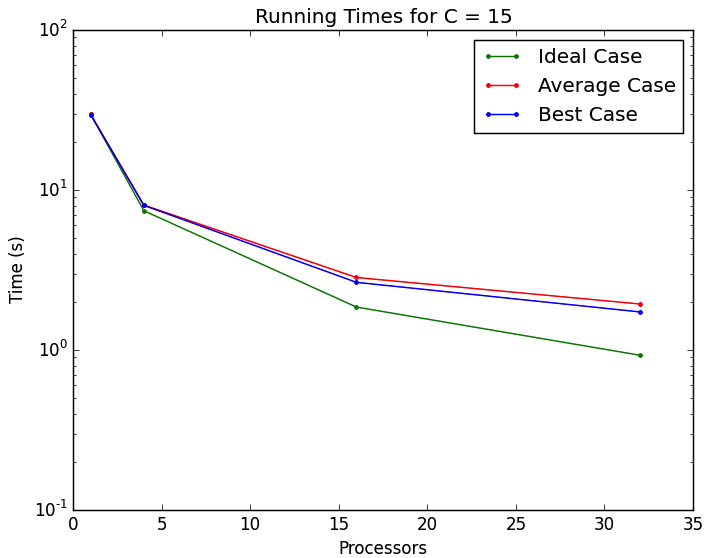
\includegraphics[width=.93\textwidth]{../2 Analysis/15_.png}
        \caption{Balanced Workload}
        \label{fig:balanced}
      \end{subfigure}%
      \begin{subfigure}{.5\textwidth}
        \centering
        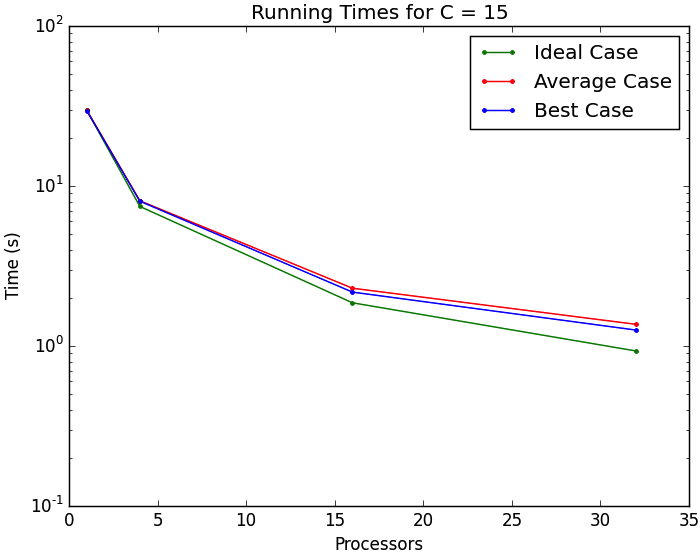
\includegraphics[width=.93\textwidth]{../2 Analysis/15_unfair.png}
        \caption{Unbalanced Workload}
        \label{fig:unbalanced}
      \end{subfigure}
      \caption{Logarithmic plot of times for different number of processors}
    \end{figure}

    Now, to analyze both SpeedUp and Efficiency, we can see the plots shown in Figures \ref{fig:SpeedUp} and \ref{fig:Efficiency}, in which we can find again the ideal case, for balanced and unbalanced node exploration. The same patterns appear here. We can appreciate that the parallelization is good enough to render a quasi linear speedup which in a load balancing algorithm seems good enough. However, bigger data sizes and processor numbers should be ran in order to get definitive results.

    

    % Finally, it is important to notice that MPI communication does not behave as the theoretical models and therefore the results will not match perfectly to the model. Nevertheless, we have achieved successful results in the time needed to solve the problem.


    \begin{figure}[htp!]
      \centering
      \begin{subfigure}{.5\textwidth}
        \centering
        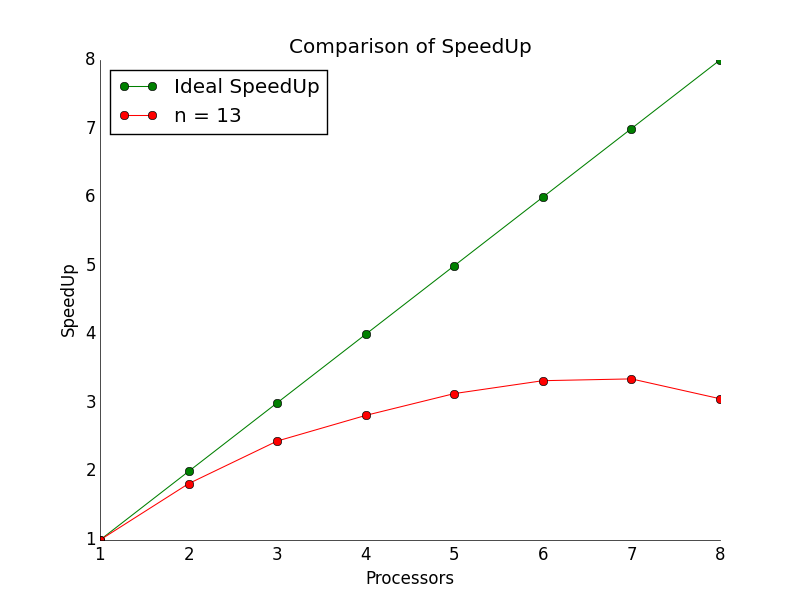
\includegraphics[width=.99\textwidth]{../2 Analysis/SpeedUp.png}
        \caption{Speed-Up}
        \label{fig:SpeedUp}
      \end{subfigure}%
      \begin{subfigure}{.5\textwidth}
        \centering
        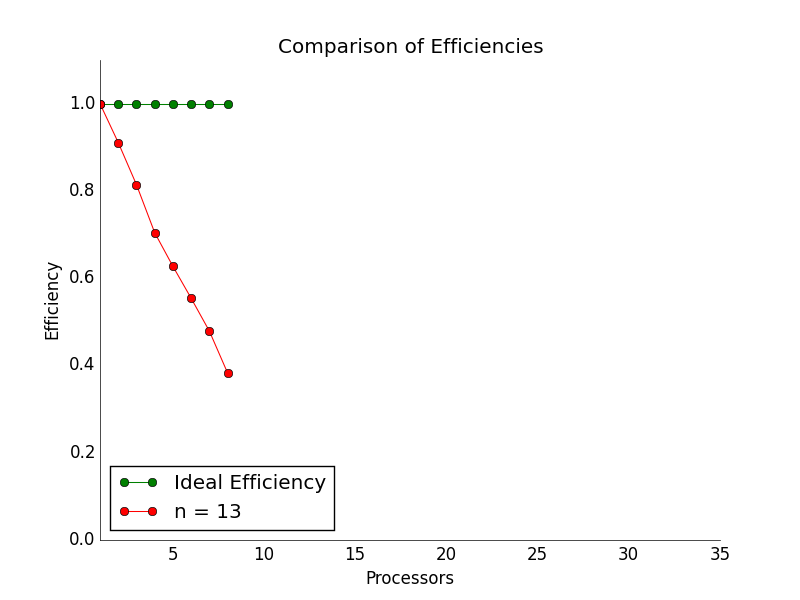
\includegraphics[width=.99\textwidth]{../2 Analysis/Efficiency.png}
        \caption{Efficiency}
        \label{fig:Efficiency}
      \end{subfigure}
      \caption{Speed-Up and Efficiency plots for the ideal case, Balanced and Unbalanced Workload}
    \end{figure}

    \begin{figure}[htp!]
      \centering
      \begin{subfigure}{.5\textwidth}
        \centering
        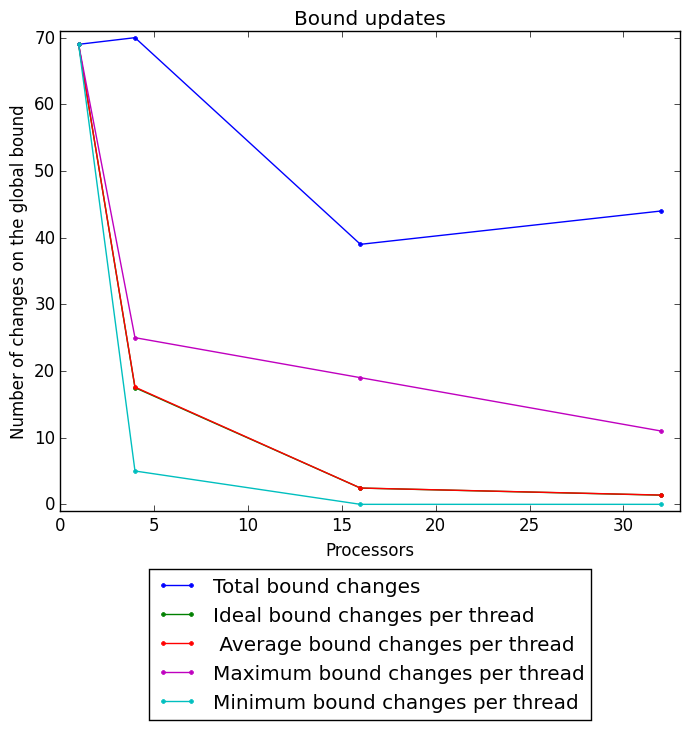
\includegraphics[width=.99\textwidth]{../2 Analysis/Load/BFS_changes.png}
        \caption{Changes over the global bound}
        \label{fig:changes}
      \end{subfigure}%
      \begin{subfigure}{.5\textwidth}
        \centering
        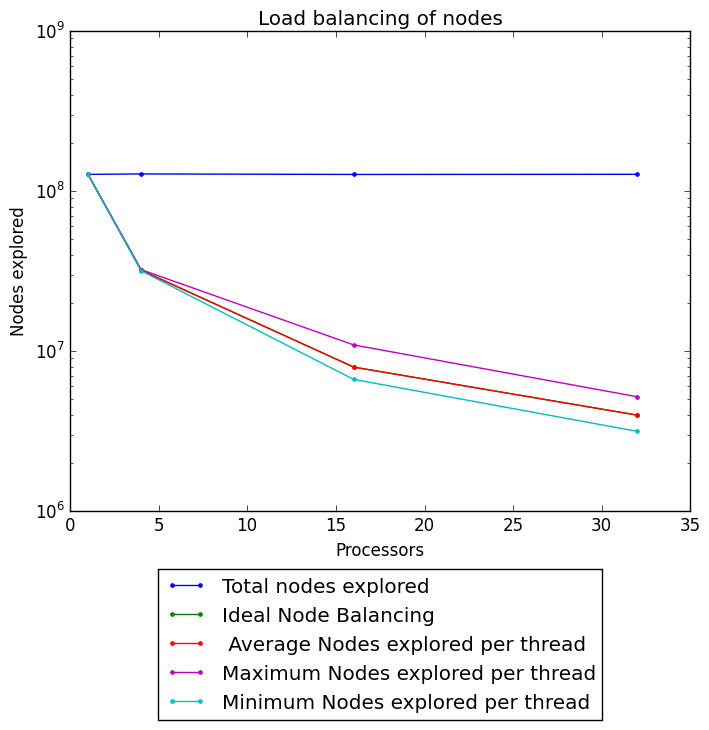
\includegraphics[width=.99\textwidth]{../2 Analysis/Load/BFS_paths.png}
        \caption{Nodes explored per thread}
        \label{fig:paths}
      \end{subfigure}%

      \vspace{2em}

      \centering
      \begin{subfigure}{.5\textwidth}
        \centering
        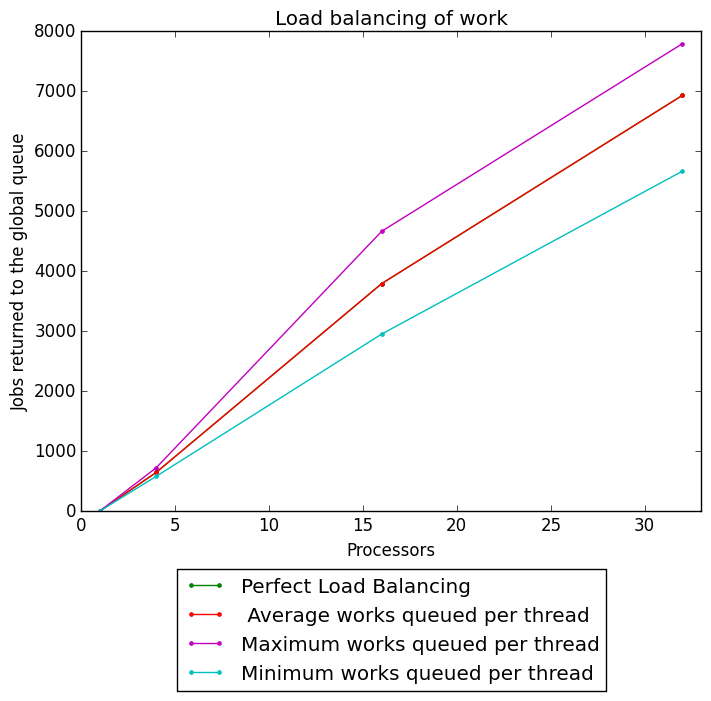
\includegraphics[width=.99\textwidth]{../2 Analysis/Load/BFS_pushes.png}
        \caption{Pushes into the global queue per proc.}
        \label{fig:pushes}
      \end{subfigure}%
      \begin{subfigure}{.5\textwidth}
        \centering
        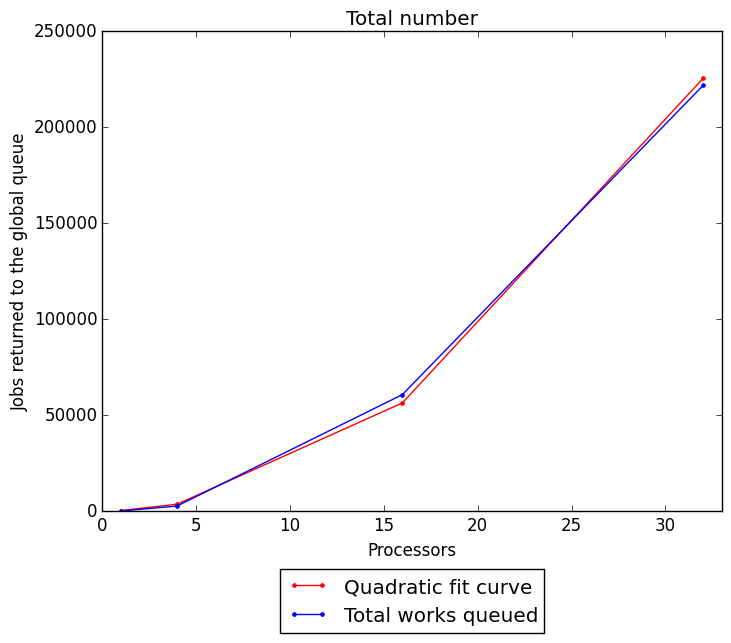
\includegraphics[width=.99\textwidth]{../2 Analysis/Load/BFS_total_pushes.png}
        \caption{Total number of pushes into the global queue}
        \label{fig:total}
      \end{subfigure}%
      \caption{Workload balancing measurements for different number of processors}
    \end{figure}

\newpage

    In order to analyze why the balanced workload algorithm is behaving like that, a number of measurements variables have been set up in order to keep track on the behavior for the load balancing. The variables that have been recorded were the following
    \begin{enumerate}
        \item \textbf{Changes on the global bound} - Since no matter what the algorithm we are forcing the best bound update to be done in mutual exclusion, we would want to estimate how often does it occur in order to determine if it can be slowing down the program.  As Figure \ref{fig:changes} shows, the number of updates is ridiculously low. For all of the runs, the number of changes was lower than 100, and since the number of explored nodes $N = 127065766$ is 7 orders of magnitude greater than the number of changes this should not affect the running times.

        \item \textbf{Nodes explores per thread} - This is a good estimate of how much work each processor is taking per execution. The sum of the explored nodes should not exceed the serial number of explored nodes ($N = 127065766$) and ideally for $p$ processors we should expect $N/p$ explored nodes per processors. This is shown in Figure \ref{fig:paths}. Since we are plotting logarithmically, the results shown look good. The load is being balanced and no processor is doing a excessive amount of work.

        \item \textbf{Job pushes to the global queue} - The previous variable measured the \emph{worker} load balancing while this one is going to measure the way the \emph{manager role} is being balanced through the processors, since as we said earlier we are using a distributed manager scheme.

        In Figure \ref{fig:pushes} we can appreciate two facts, the first is that the number of pushes into the queue per processor grows as the number of processors increases. This is logical, since having more processors implies that more dead-ends will produce more empty stacks and therefore more idle processors than need work to be sent to them. The second fact is that the workload seems balanced, although is not as good balanced as the path exploring task, we still get an average coincidental to the ideal.

        Finally the biggest clue about the surprising speed of the unbalanced approach comes from the analysis of Figure \ref{fig:total}. As we can see the total amount of pushes into the queue grows as a quadratic function, more specifically $F(p) \approx 220p^2$. This implies that the communication overhead complexity is $\Theta(p^2)$ and therefore we will spend more time balancing the work than just doing the work in an unbalanced fashion. This explains the results obtained before.

    \end{enumerate}

    As an end note just to remark that the unbalanced algorithm could do better in this case since we initialized the queue with three levels of recursion which usually is a big enough number for a realistic number of processors. Namely, had we chosen to initialize the queue with $p$ nodes, the unbalanced algorithm would have behaved much worse than the balanced one. Also, it has to be taken into account the fact that we are only using a strict set of data points, which coincidentally have distances that almost self balance the problem. Given a more complex set of data points, probably the scaling for the unbalanced algorithm could be worse than for the balanced algorithm.

\newpage
\section{Correctness}

    Finally, we need to check that the algorithm produced the correct results. For all the different runs with varying number of processors, the algorithm always outputted the correct answer, guaranteeing us the correctness of the implementation. In Figure \ref{fig:best} we can see the visualization on the solution. (Note that although euclidean distances are plotted, those are not the distances that have been used in the algorithm)
    \begin{align}
    \begin{split}
      \text{path} &= [0, 13, 9, 1, 8, 14, 7, 2, 3, 4, 11, 6, 10, 12, 5]\\
      \text{cost} &= 782.989290
    \end{split}
    \end{align}

    \begin{figure}[htp!]
      \centering
        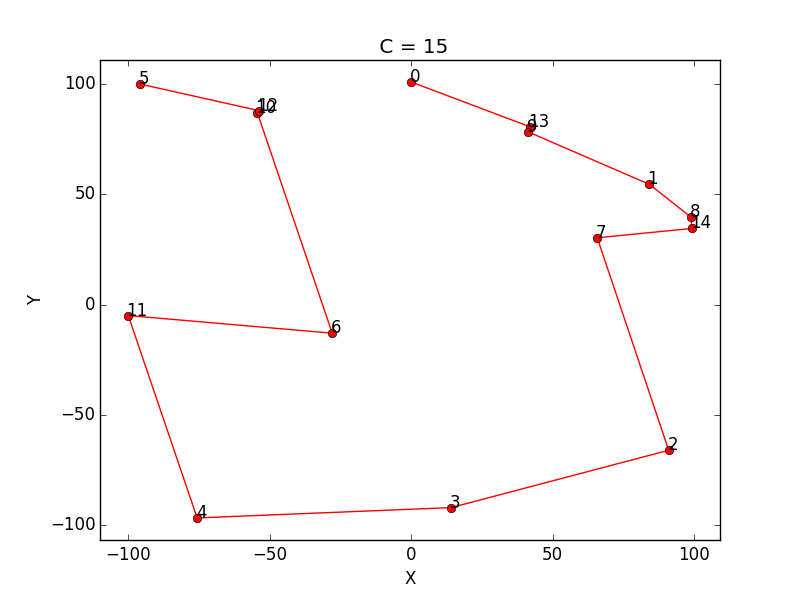
\includegraphics[width=.79\textwidth]{../2 Analysis/C15.png}
        \caption{Shortest Path}
        \label{fig:best}
    \end{figure}




\end{document}
